\documentclass[]{scrreprt}
\usepackage{amsmath,amsfonts,graphicx}

\def\species{\mathrm{sp}}
\def\phase{\mathrm{ph}}
\def\massfrac{\chi}
\def\flux{\mathbf{F}}
\def\darcyvel{\mathbf{v}}
\def\energydens{\mathcal{E}}
\def\d{\mathrm{d}}

\newcommand{\uo}{\mbox{UO\textsubscript{2}}\xspace}

\setcounter{secnumdepth}{3}


\begin{document}


\title{Poroelasticitiy Tests}
\author{CSIRO}
\maketitle

\tableofcontents

\chapter{Introduction}

The PorousFlow module includes the ability to couple fluid flow to
solid mechanics, and thus includes poroelasticity, which is the theory
of a fully-saturated single-phase fluid with constant bulk density and
constant viscosity coupled to small-strain isotropic elasticity.

There is one important difference between the theories, however.  The
time-derivative terms of poroelasticity are
\begin{equation}
\frac{1}{M}\dot{P} + \alpha\dot{\epsilon}_{ii} \ ,
\label{eqn.poro.dt}
\end{equation}
where $M$ is the Biot modulus:
\begin{equation}
\frac{1}{M} = \frac{(1-\alpha)(\alpha - \phi)}{K} +
\frac{\phi}{K_{\mathrm{f}}} \ ,
\label{biotmod.eqn}
\end{equation}
$P$ is the fluid porepressure, $\alpha$ is the Biot coefficient,
$\epsilon_{ii}$ is the volumetric strain, $\phi$ is the porosity, $K$
is the solid (drained) bulk modulus, and $K_{\mathrm{f}}$ is the fluid
bulk modulus.  Evidently from Eqn~(\ref{biotmod.eqn}), the Biot
modulus, $M$, should evolve with time as the porosity evolves.
Indeed, the terms in Eqn~(\ref{eqn.poro.dt}) are derived from the
continuity equation $\partial (\phi\rho)/\partial t +
\phi\rho\dot{\epsilon}_{ii}$ using the evolution of $\phi$ (and that
$\rho = \rho_{0}\exp(P/K_{\mathrm{f}})$).  However, in the standard
analytical solutions of poroelasticity theory, the Biot modulus, $M$
is considered fixed.

The PorousFlow module allows porosity to vary with fluid porepressure
and volumetric strain, so usually the Biot modulus would vary too,
causing differences with the analytical solutions of poroelasticity.
Therefore, PorousFlow offers a porosity relationship that evolves
porosity in such a way as to keep $M$ fixed.  This is called {\tt
  PorousFlowPorosityHMBiotModulus}.

PorousFlow is also built with finite strains in mind, whereas
poroelasticity is not.  Therefore, in comparisons with solutions from
poroelasticity theory, either the strain should be kept small, or the
various finite-strain switches in PorousFlow should be turned off
(they are all on by default).

\chapter{Simple tests}

\section{Volumetric expansion due to increasing porepressure}

The porepressure within a fully-saturated sample is increased:
\begin{equation}
P_{\mathrm{f}} = t \ .
\end{equation}
Zero mechanical pressure is applied to the sample's exterior, so that
no Neumann BCs are needed on the sample.  No fluid flow occurs since
the porepressure is increased uniformly throughout the sample

The effective stresses should then evolve as
$\sigma_{ij}^{\mathrm{eff}} = \alpha t \delta_{ij}$, and the
volumetric strain $\epsilon_{00}+\epsilon_{11}+\epsilon_{22} = \alpha
t/K$.  MOOSE produces this result correctly.

\section{Undrained oedometer test}

A cubic single-element fully-saturated sample has roller BCs applied
to its sides and bottom.  All the sample's boundaries are impermeable.
A downwards (normal) displacement, $u_{z}$, is applied to its
top, and the rise in porepressure and effective stress is observed.
(Here $z$ denotes the direction normal to the top face.)  There is
no fluid flow in the single element.

Under these conditions, assuming constant porosity, and denoting the
height ($z$ length) of the sample by $L$:
\begin{eqnarray}
P_{\mathrm{f}} & = & -K_{f}\log(1 - u_{z}) \ , \nonumber \\
\sigma_{xx}^{\mathrm{eff}} & = & (K - \mbox{$\frac{2}{3}$}G)u_{z}/L \ , \nonumber \\
\sigma_{zz}^{\mathrm{eff}} & = & (K + \mbox{$\frac{4}{3}$}G)u_{z}/L \ .
\end{eqnarray}

\section{Porepressure generation of a confined sample}

A single-element fully-saturated sample is constrained on all sides
and its boundaries are impermeable.  Fluid is pumped into the sample
via a source $s$ (kg.s$^{-1}$.m$^{-3}$) and the rise
in porepressure is observed.

Denoting the strength of the source by $s$ (units are s$^{-1}$), the expected result is
\begin{eqnarray}
\mbox{fluid mass} & = & \mbox{fluid mass}_{0} + st \ , \nonumber \\
\sigma_{ij}^{\mathrm{eff}} & = & 0 \ , \nonumber \\
P_{\mathrm{f}} & = & K_{\mathrm{f}}\log(\rho\phi/\rho_{0}) \ , \nonumber
\\
\rho & = & \rho_{0}\exp(P_{\mathrm{f}}/K_{f}) \ , \nonumber \\
\phi & = & \alpha + (\phi_{0}-\alpha)\exp\left(
P_{\mathrm{f}}(\alpha - 1)/K\right) \ . \\
\end{eqnarray}
Here $K$ is the solid bulk modulus.

\section{Porepressure generation of an unconfined sample}

A single-element fully-saturated sample is constrained on all sides,
except its top.  All its boundaries are impermeable.  Fluid is pumped
into the sample via a source $s$ (kg.s$^{-1}$.m$^{-3}$)) and the rise
in the top surface, the porepressure, and the stress are observed.

Regardless of the evolution of porosity, the following ratios result
\begin{eqnarray}
\sigma_{xx}/\epsilon_{zz} & = & K - 2G/3 \ , \nonumber \\
\sigma_{zz}/\epsilon_{zz} & = & K + 4G/3 \ , \nonumber \\
P/\epsilon_{zz} & = & (K + 3G/3 + \alpha^{2}M)/\alpha - \alpha M \ .
\end{eqnarray}
where $K$ is the undrained bulk modulus, $G$ the shear modulus,
$\alpha$ the Biot coefficient, and $M$ is the initial Biot modulus.
MOOSE produces these results when using the {\tt
  PorousFlowPorosityHM} material.


However, if the Biot modulus, $M$, is held fixed as the porosity
evolves, and the source is
\begin{equation}
s = S \rho_{0}\exp(P/K_{\mathrm{f}}) \ ,
\end{equation}
with $S$ being a {\em constant} volumetric source
(m$^{3}$.s$^{-1}$.m$^{-3}$) then
\begin{eqnarray}
\epsilon_{zz} & = & \frac{\alpha M s t}{K + 4G/3 + \alpha^{2}M} \ ,
\nonumber \\
P & = & M(st - \alpha\epsilon_{zz}) \ , \nonumber \\
\sigma_{xx} & = & (K - 2G/3)\epsilon_{zz} \ , \nonumber \\
\sigma_{zz} & = & (K + 4G/3)\epsilon_{zz} \ .
\end{eqnarray}
MOOSE produces these results when using the {\tt
  PorousFlowPorosityHMBiotModulus} material.

\chapter{Terzaghi consolidation}

This is documented at {\tt
  http://mooseframework.org/wiki/PhysicsModules/TensorMechanics/TensorMechanicsBasics/PoroMechanics/}.
The PorousFlow Material {\tt PorousFlowPorosityHMBiotModulus} must be used.

\chapter{Mandel's consolidation of a drained medium}

A sample's dimensions are $-a \leq x \leq a$ and $-b \leq y \leq b$,
and it is in plane strain (no $z$ displacement).  It is squashed with
constant normal force by impermeable, frictionless plattens on its top
and bottom surfaces (at $y = \pm b$).  Fluid is allowed to leak out
from its sides (at $x = \pm a$), but all other surfaces are
impermeable.  This is called Mandel's problem and it is shown
graphically in Fig~\ref{mandel_setup.fig}

\begin{figure}[htb]
\begin{center}
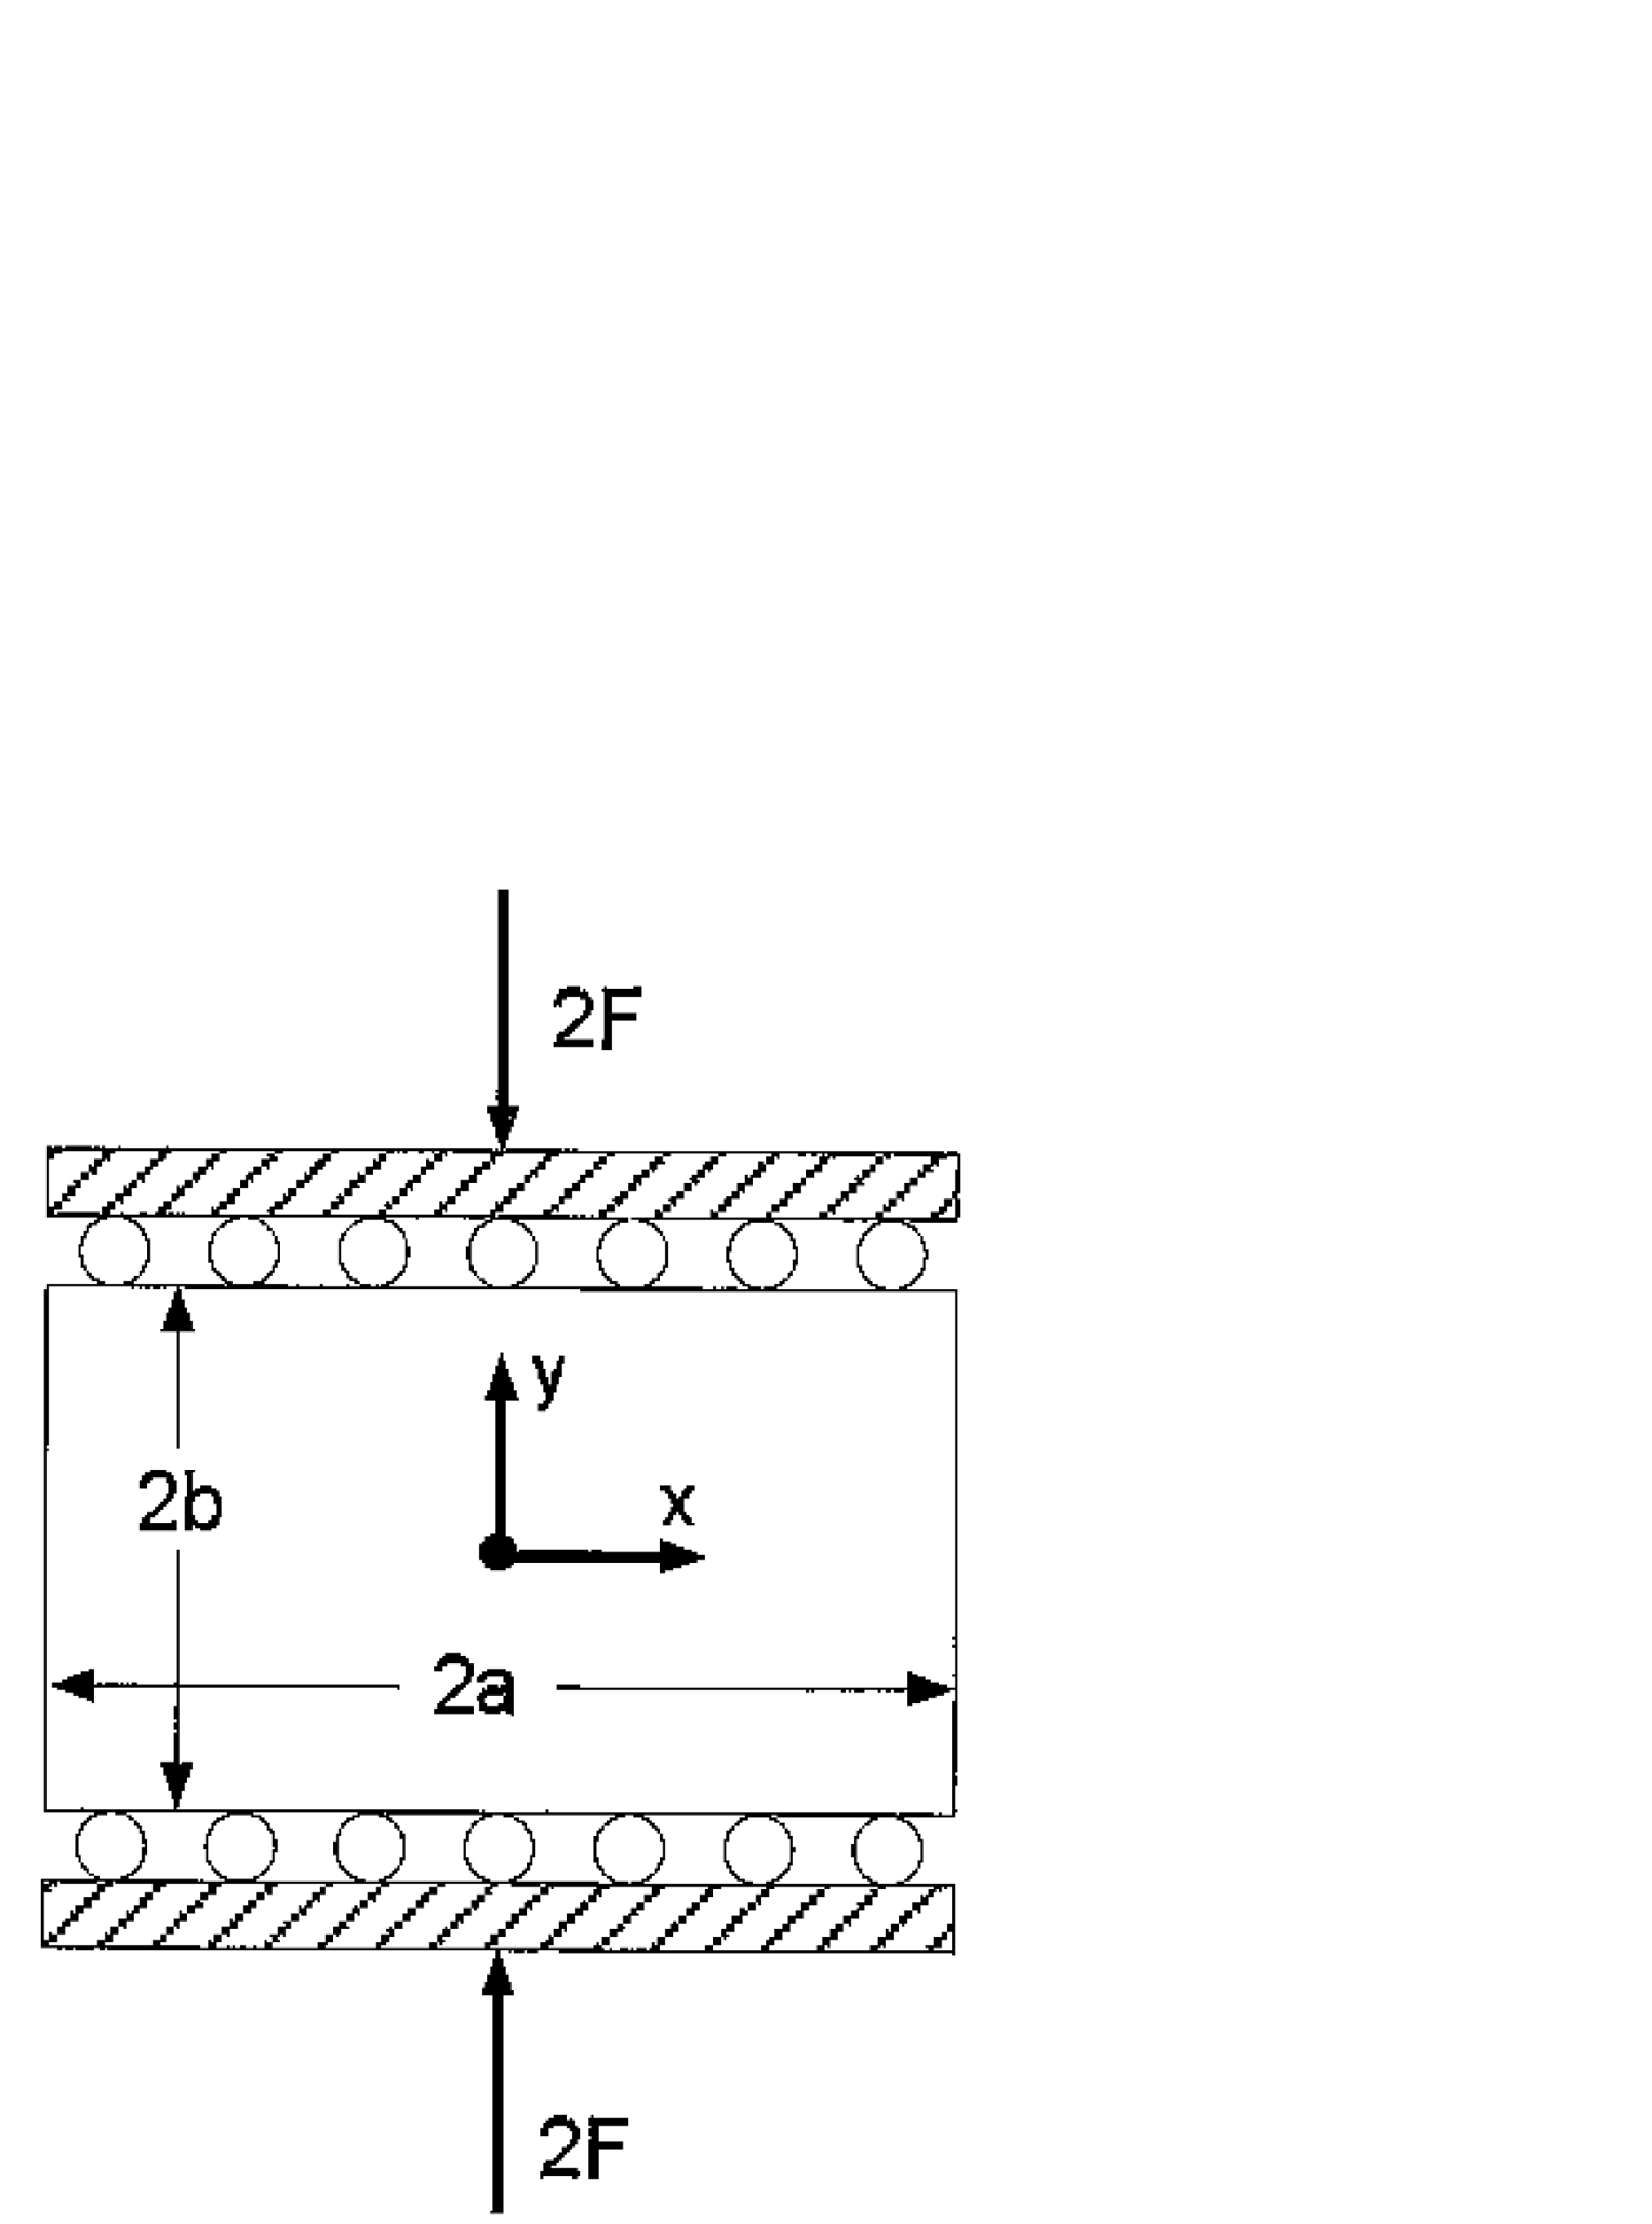
\includegraphics[width=8cm]{mandel_setup.pdf}
\caption{The setup of the Mandel experiment: a force $F$ squashes a
  porous material with impermeable plattens.  This causes fluid to
  seep from the material.}
\label{mandel_setup.fig}
\end{center}
\end{figure}

The interesting feature of this problem (apart from that it can be
solved analytically) is that the porepressure in the sample's center
actually increases for a short time after application of the force.
This is because the leakage of the fluid from the sample's sides
causes an apparent softening of the material near those sides.  This
means stress concentrates towards the sample's center which causes an
increase in porepressure.  Of course, eventually the fluid totally
drains from the sample, and the porepressure is zero.  As the fluid
drains from the sample's sides the plattens move slowly towards each
other.

The solution for porepressure and displacements is given in: AHD Cheng
and E Detournay ``A direct boundary element method for plane strain
poroelasticity'' International Journal of Numerical and Analytical
Methods in Geomechanics 12 (1988) 551-572.  The solution involves
rather lengthy infinite series, so I will not write it here.

As is common in the literature, this is simulated by considering the
quarter-sample, $0\leq x \leq a$ and $0\leq y\leq b$, with
impermeable, roller BCs at $x=0$ and $y=0$ and $y=b$.  Porepressure is
fixed at zero on $x=a$.  Porepressure and displacement are initialised
to zero.  Then the top ($y=b$) is moved downwards with prescribed
velocity, so that the total force that is induced by this downwards
velocity is fixed.  The velocity is worked out by solving Mandel's
problem analytically, and the total force is monitored in the
simulation to check that it indeed remains constant.

The simulations in the PorousFlow test suite use 10 elements in the
$x$ direction and 1 in the $y$ direction.  Four types of simulation
are run:
\begin{enumerate}
\item HM.  This uses standard PorousFlow Materials and Kernels, in
  particular it uses the ``HM'' porosity relationship.  This is not
  expected to agree perfectly with the analytical solutions because:
  the solutions assume constant Biot modulus.
\item constM.  This is identical to the HM case, save that it uses a
  porosity evolution law that keeps the Biot modulus fixed.  It is
  therefore expected to agree with the analytical solutions.
\item FullSat.  This uses the FullySaturated versions of the fluid
  mass time derivative and the fluid flux.  In this case the Biot
  modulus is kept fixed, so it is expected to agree with the
  analytical solutions.
\item FullSatVol.  This uses the FullySaturated versions of the fluid
  mass time derivative and the fluid flux, and does not multiply by
  the fluid density.  Therefore this version is identical to what is
  usually implemented in poro-elastic codes.  It is linear and
  therefore converges in only one iteration.  In this case the Biot
  modulus is kept fixed, so it is expected to agree with the
  analytical solutions.
\end{enumerate}
Of course there are minor discrepancies between the last three and the
analytical solution that are brought about through spatial and
temporal discretisation errors.  The figures below present the
results.

\begin{figure}[htb]
\begin{center}
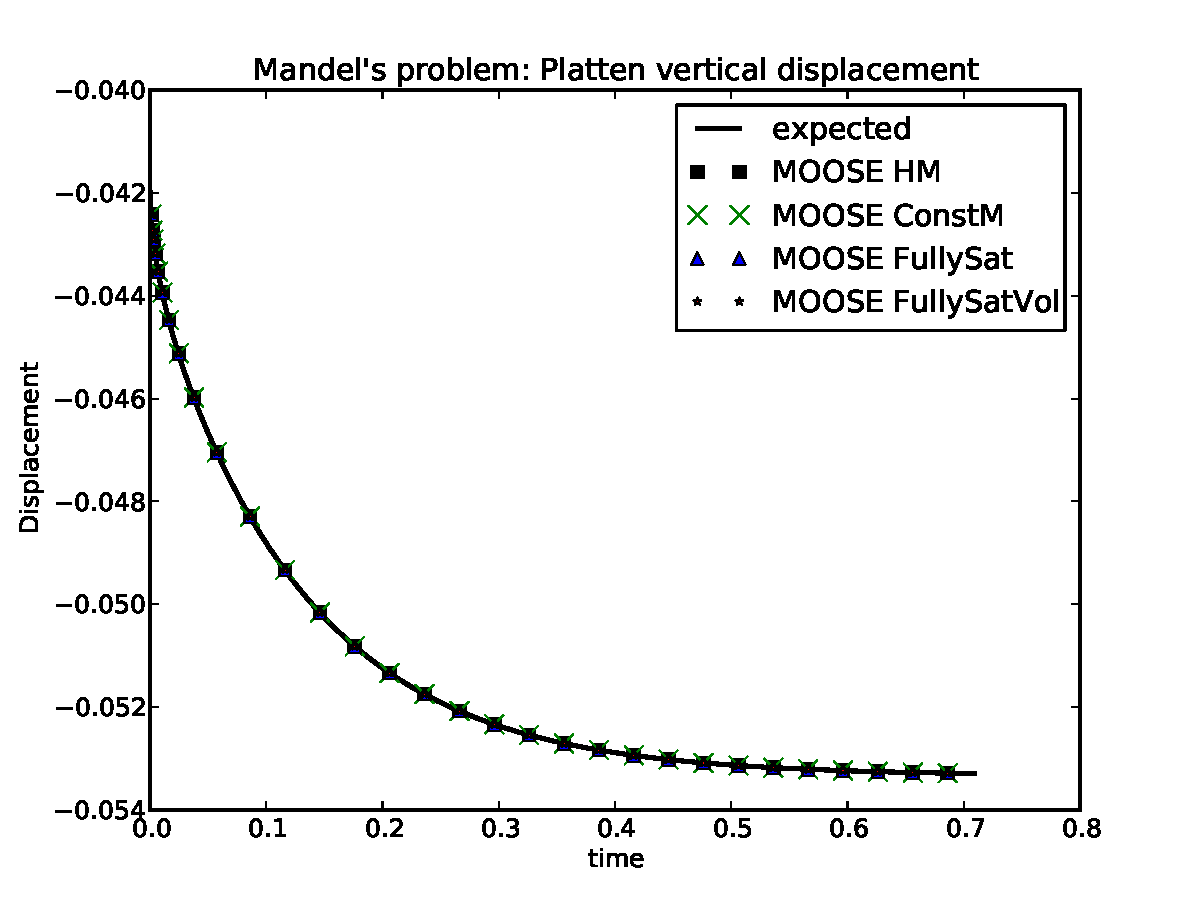
\includegraphics[width=11cm]{mandel_ver_disp.pdf}
\caption{The vertical displacement of the platten as a function of time.}
\label{mandel_ver_disp.fig}
\end{center}
\end{figure}

\begin{figure}[htb]
\begin{center}
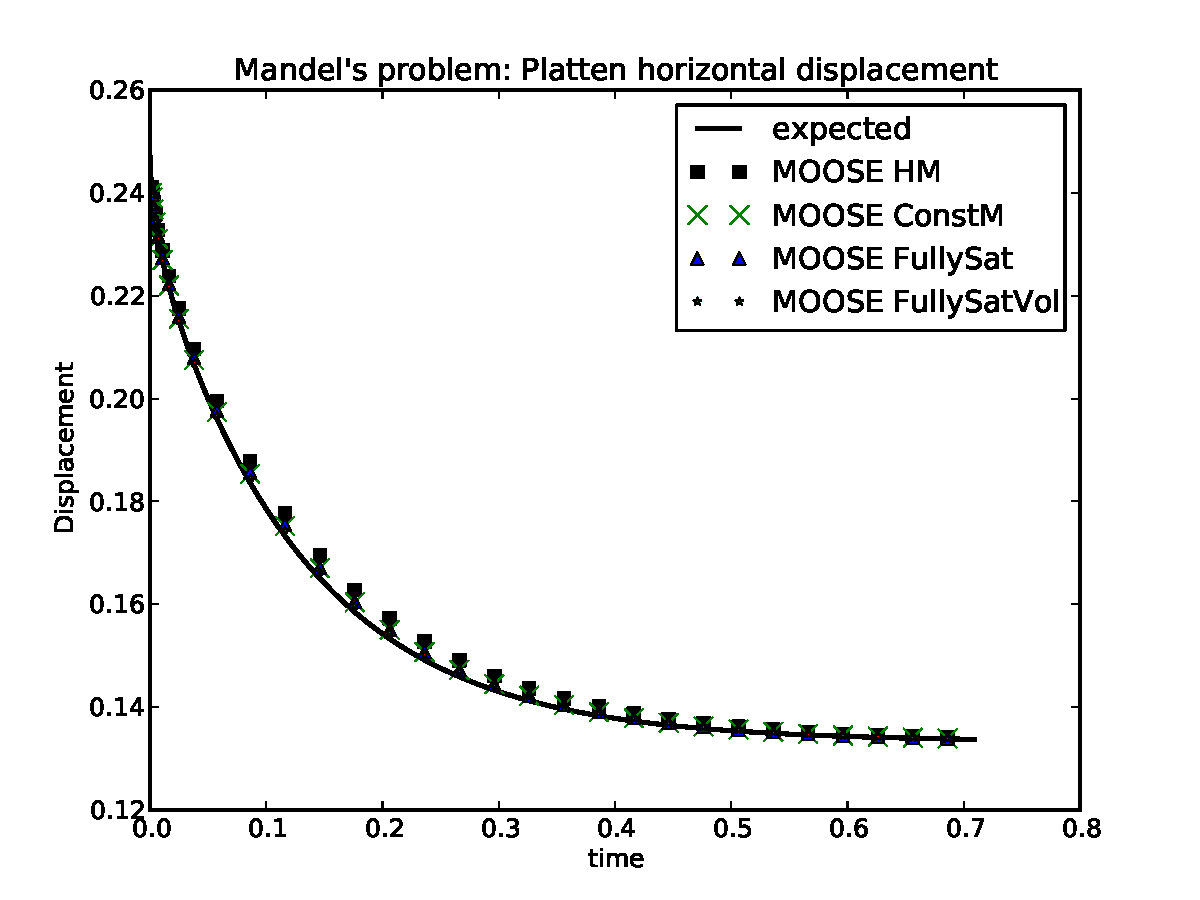
\includegraphics[width=11cm]{mandel_hor_disp.pdf}
\caption{The horizontal displacement of the material at $(x,y) = (a,
  b)$ as a function of time.}
\label{mandel_hor_disp.fig}
\end{center}
\end{figure}


\begin{figure}[htb]
\begin{center}
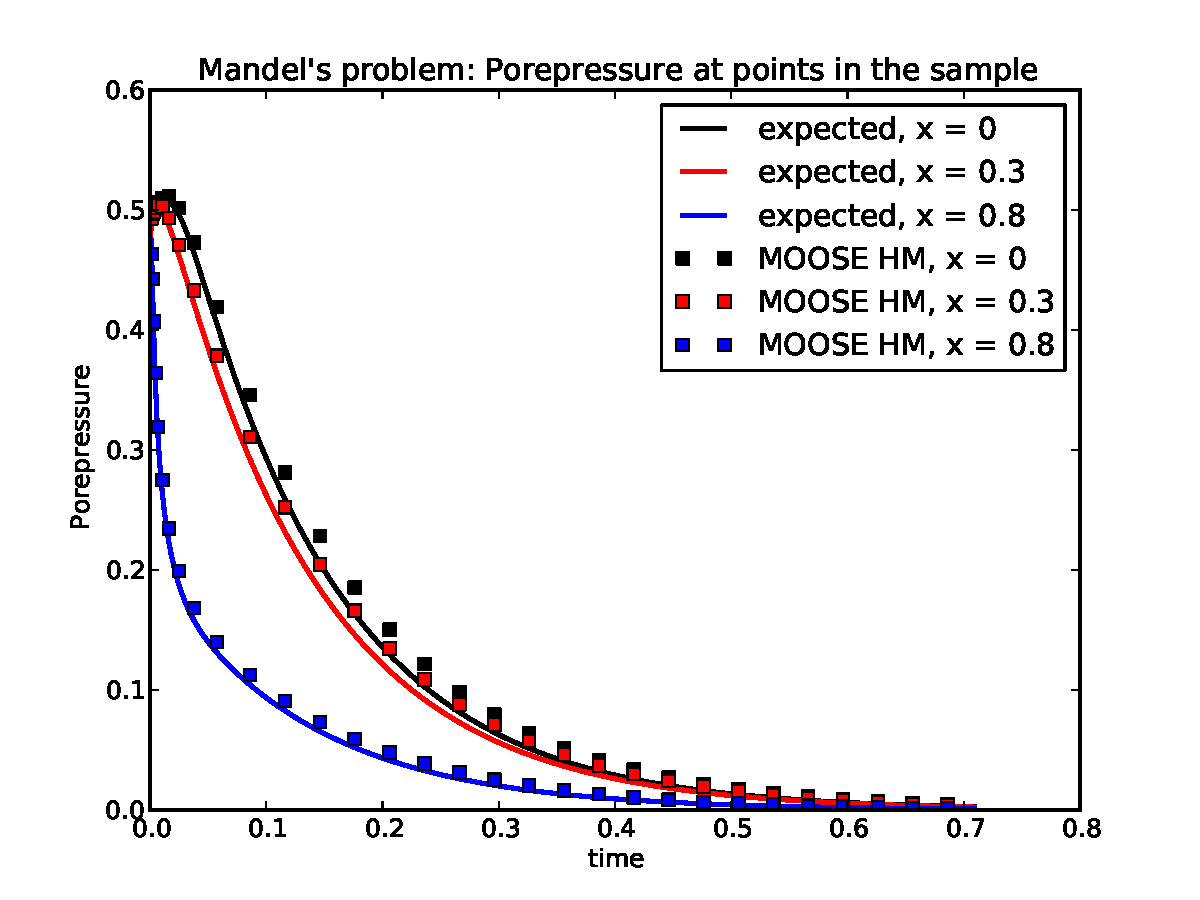
\includegraphics[width=11cm]{mandel_HM.pdf}
\caption{The porepressure at various points in the sample in the HM
  model with $a=1$.}
\label{mandel_HM.fig}
\end{center}
\end{figure}


\begin{figure}[htb]
\begin{center}
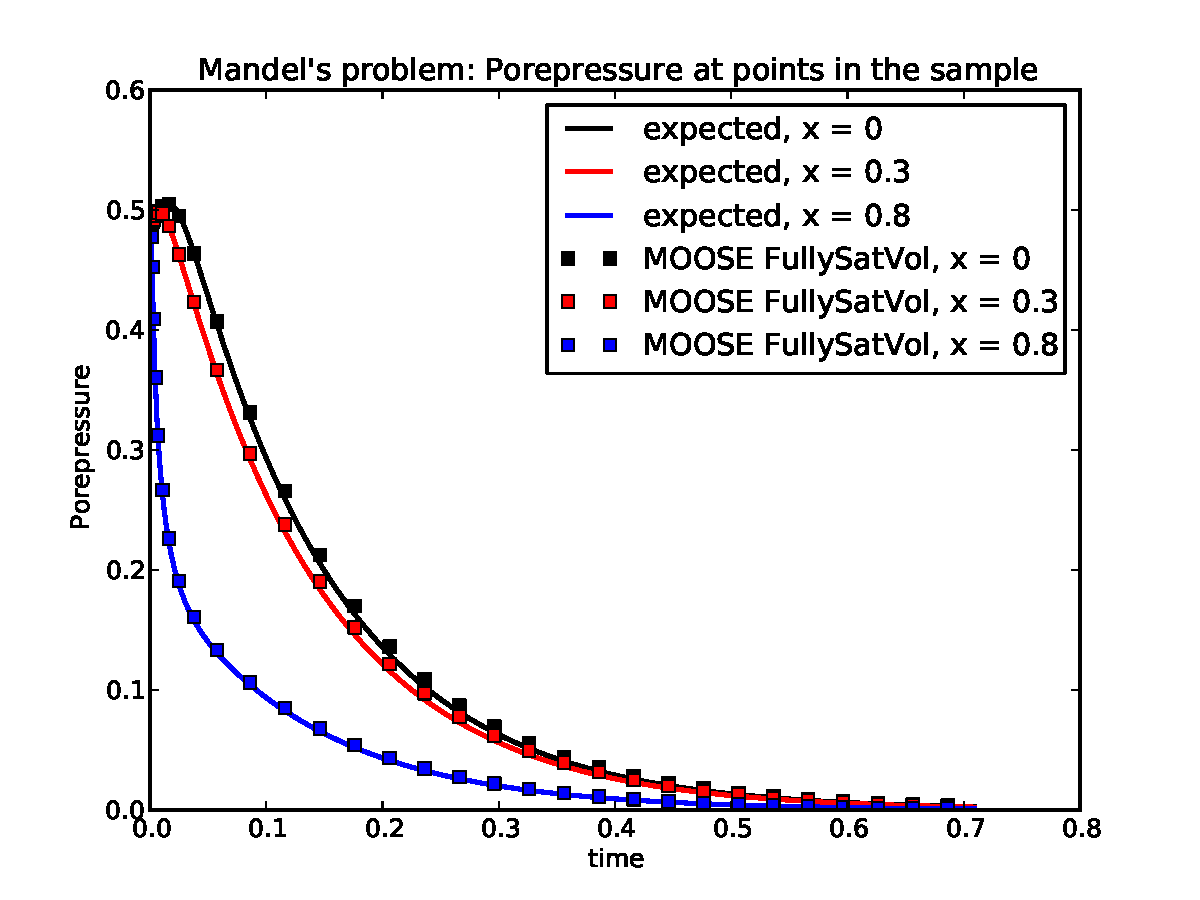
\includegraphics[width=11cm]{mandel_FSV.pdf}
\caption{The porepressure at various points in the sample in the FullSatVol
  model with $a=1$.}
\label{mandel_FSV.fig}
\end{center}
\end{figure}

\begin{figure}[htb]
\begin{center}
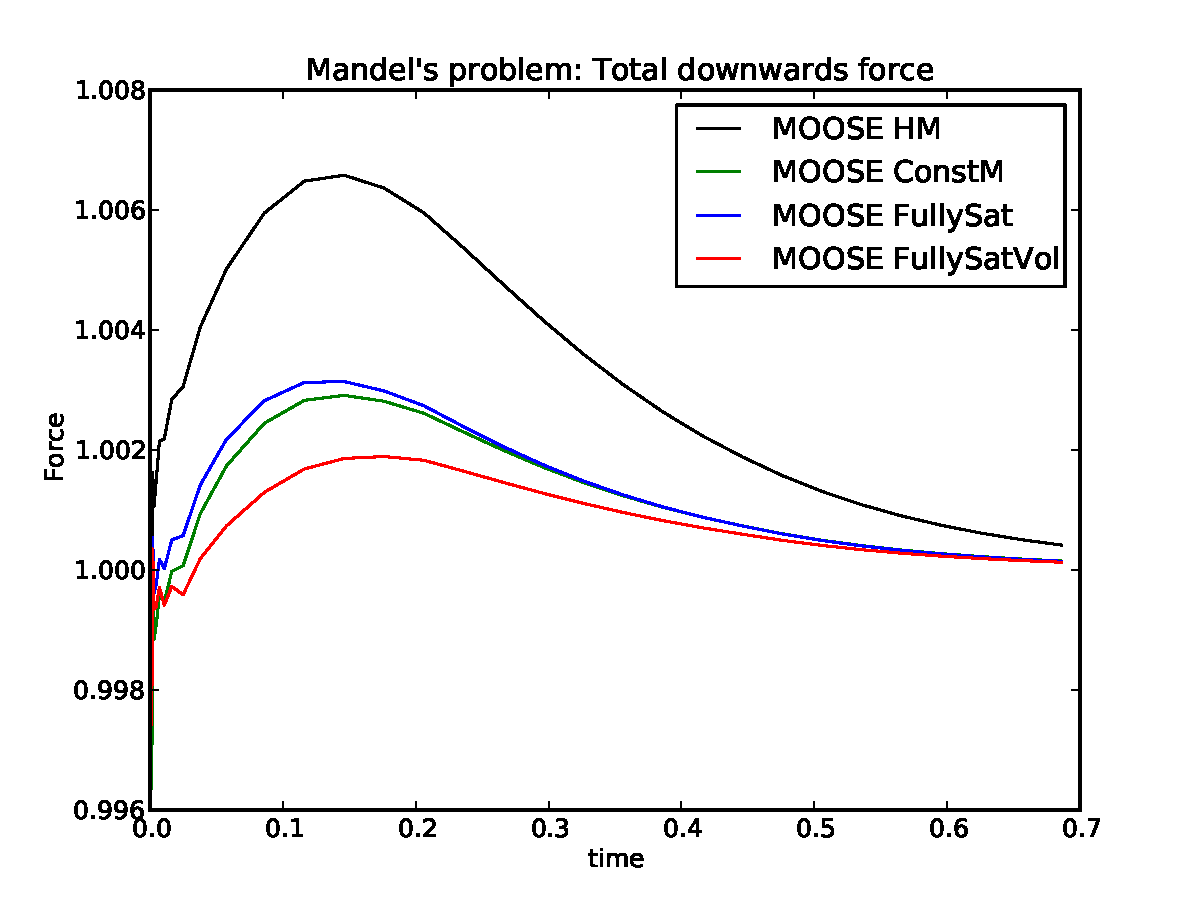
\includegraphics[width=11cm]{mandel_force.pdf}
\caption{The total downwards force on the platten as a function of
  time.  This should be unity.}
\label{mandel_force.fig}
\end{center}
\end{figure}









\end{document}

